\documentclass[aspectratio=169,11pt]{beamer}
\usetheme[progressbar=frametitle,numbering=fraction]{metropolis}
\usepackage[T1]{fontenc}
\usepackage[utf8]{inputenc}
\usepackage[polish]{babel}
\usepackage{booktabs}
\usepackage{tikz}
\usetikzlibrary{arrows.meta,positioning,calc}

\definecolor{navy}{RGB}{20,40,120}
\definecolor{hdfs}{RGB}{230,140,40}
\definecolor{baza}{RGB}{60,140,90}
\setbeamercolor{frametitle}{bg=navy}
\setbeamercolor{progress bar}{fg=hdfs}
\newcommand{\kod}[1]{\texttt{#1}}

% liczby i tabele generuje sprawozdanie_latex/generuj.py z plików w wyniki/
\newcommand{\tabBlunder}{%
\begin{tabular}{llrrr}
\toprule
Tempo & Elo & Z czasem & Pod flagą & Wzrost \\
\midrule
ultrabullet & $<$1200 & 24,8\% & 44,4\% & +79\% \\
ultrabullet & 1200 & 25,3\% & 38,4\% & +52\% \\
ultrabullet & 1600 & 22,1\% & 34,4\% & +56\% \\
ultrabullet & 2000 & 20,2\% & 31,7\% & +57\% \\
ultrabullet & 2400+ & 16,7\% & 29,1\%* & +75\% \\
\addlinespace[2pt]
bullet & $<$1200 & 22,6\% & 32,8\% & +45\% \\
bullet & 1200 & 19,7\% & 29,7\% & +51\% \\
bullet & 1600 & 18,2\% & 27,7\% & +52\% \\
bullet & 2000 & 16,2\% & 26,6\% & +64\% \\
bullet & 2400+ & 13,4\% & 26,7\% & +99\% \\
\addlinespace[2pt]
blitz & $<$1200 & 23,2\% & 33,8\% & +45\% \\
blitz & 1200 & 18,7\% & 29,4\% & +57\% \\
blitz & 1600 & 16,1\% & 26,8\% & +67\% \\
blitz & 2000 & 12,9\% & 24,0\% & +86\% \\
blitz & 2400+ & 10,1\% & 22,4\% & +121\% \\
\addlinespace[2pt]
rapid & $<$1200 & 25,5\% & 38,1\% & +49\% \\
rapid & 1200 & 19,3\% & 31,7\% & +64\% \\
rapid & 1600 & 15,8\% & 27,3\% & +73\% \\
rapid & 2000 & 12,3\% & 24,8\% & +102\% \\
rapid & 2400+ & 8,4\% & 20,7\%* & +147\% \\
\addlinespace[2pt]
classical & $<$1200 & 27,8\% & 0,0\%* & -100\% \\
classical & 1200 & 20,7\% & 17,3\%* & -16\% \\
classical & 1600 & 14,6\% & 22,7\%* & +55\% \\
classical & 2000 & 9,8\% & 22,0\%* & +125\% \\
\addlinespace[2pt]
\bottomrule
\end{tabular}}

\newcommand{\tabComeback}{%
\begin{tabular}{lrr}
\toprule
Tempo & Udział & $n$ \\
\midrule
ultrabullet & 77,2\%* & 1850 \\
bullet & 55,7\% & 49770 \\
blitz & 47,2\% & 104385 \\
rapid & 45,9\% & 73355 \\
classical & 40,4\% & 4394 \\
\bottomrule
\end{tabular}}

\newcommand{\tabThink}{%
\begin{tabular}{llrrr}
\toprule
Tempo & Elo & 0--2 s & 2--10 s & 10+ s \\
\midrule
blitz & $<$1200 & 65,6 & 91,4 & 123,4 \\
blitz & 1200 & 55,7 & 75,8 & 103,5 \\
blitz & 1600 & 50,6 & 67,3 & 92,6 \\
blitz & 2000 & 44,5 & 55,5 & 77,8 \\
blitz & 2400+ & 40,5 & 45,8 & 63,9 \\
\addlinespace[2pt]
bullet & $<$1200 & 80,0 & 103,6 & 126,1 \\
bullet & 1200 & 68,2 & 93,0 & 117,9 \\
bullet & 1600 & 64,0 & 88,9 & 111,9 \\
bullet & 2000 & 60,7 & 83,5 & 98,1 \\
bullet & 2400+ & 57,2 & 75,6 & 109,0* \\
\addlinespace[2pt]
\bottomrule
\end{tabular}}

\graphicspath{{../sprawozdanie_latex/figures/}}

\title{BigData Chess Analyzer}
\subtitle{Partie z Lichess w HDFS, Hadoop Streaming i MongoDB}
\author{Jakub Balicki}
\institute{Big Data, projekt 1}
\date{listopad 2026}

\begin{document}

\maketitle

\begin{frame}{Problem i dane}
\begin{columns}[T]
\column{0.52\textwidth}
\textbf{Pytania}
\begin{enumerate}
\item Czy pod presją czasu (zegar $\le$ 10 s) robi się więcej błędów?
\item Jak często wygrywa ktoś, kto przegrywał o 2 piony?
\item Czy dłuższy namysł daje lepszy ruch?
\end{enumerate}
\column{0.45\textwidth}
\textbf{Dane: Lichess Open Database}
\begin{itemize}
\item wrzesień 2026, licencja CC0
\item \textbf{5,5 GB} PGN po rozpakowaniu
\item \textbf{\nGames} partii, \nMapInput{} linii
\item zegar \kod{[\%clk]} przy każdym ruchu, ocena silnika \kod{[\%eval]} w ok.\ 10\% partii
\end{itemize}
\end{columns}
\vspace{0.6em}
{\small\kod{1. e4 \{ [\%eval 0.17] [\%clk 0:03:00] \} 1... c5 \{ [\%eval 0.19] [\%clk 0:02:58] \}}}
\end{frame}

\begin{frame}{Architektura}
\centering
\begin{tikzpicture}[font=\sffamily\scriptsize, node distance=0.45cm and 0.5cm,
  box/.style={draw, rounded corners=2pt, align=center, minimum height=1.0cm, text width=2.1cm, fill=navy!6},
  h/.style={box, fill=hdfs!20}, d/.style={box, fill=baza!18}, arr/.style={-{Stealth[length=2mm]}, thick}]
\node[box] (l) {Lichess\\\kod{.pgn.zst}};
\node[box, right=of l] (p) {\kod{download.py}\\PGN 5,5 GB};
\node[h, right=of p] (r) {HDFS\\8 części};
\node[h, right=of r] (m) {Hadoop Streaming\\3 joby};
\node[h, right=of m] (o) {HDFS\\wyniki (TSV)};
\node[box, below=1.3cm of o] (ch) {wykresy\\matplotlib};
\node[d, below=1.3cm of m] (atl) {MongoDB Atlas\\\kod{mongodb+srv}};
\node[d, below=1.3cm of r] (loc) {MongoDB lokalna\\TLS + SCRAM};
\node[box, below=1.3cm of p, fill=gray!12] (f) {dodatek: scraping\\ratings.fide.com};
\draw[arr] (l) -- (p); \draw[arr] (p) -- (r); \draw[arr] (r) -- (m); \draw[arr] (m) -- (o);
\draw[arr] (o) -- (ch);
\draw[arr] (o.south) -- ++(0,-0.6) -| (atl.north);
\draw[arr] (o.south) -- ++(0,-0.6) -| (loc.north);
\node[font=\sffamily\tiny, fill=white, inner sep=1pt] at ($(m.south)!0.5!(atl.north)$) {upsert};
\draw[arr, dashed] (f) -- (loc);
\end{tikzpicture}
\vspace{0.8em}

Całość: \kod{./run\_all.sh} (pełne dane) albo \kod{./run\_all.sh -{}-probka} (50 MB, 2 min).\\
Docker: \kod{apache/hadoop:3.4.3} (HDFS + YARN) i \kod{mongo:7.0.45}.
\end{frame}

\begin{frame}{HDFS i podział na 8 części}
\begin{itemize}
\item Hadoop tnie plik na bloki po 128 MB bez patrzenia na treść, a partia PGN to kilkanaście linii: granica bloku przecięłaby partię.
\item \kod{split\_pgn.py} dzieli plik na \textbf{8 części po ok.\ 690 MB}, zawsze tuż przed \kod{[Event "}.
\item W jobie \kod{split.minsize} = 2 TB: każda część to dokładnie \textbf{1 split = 1 mapper}.
\item Ponowna wysyłka pomijana, gdy w HDFS są już części o tych samych rozmiarach.
\end{itemize}
\vspace{0.5em}
{\small\kod{\$ hdfs dfs -du -s -h /user/chess/raw/lichess\_2026-09}\\
\kod{5.1 G  5.1 G  /user/chess/raw/lichess\_2026-09}}
\end{frame}

\begin{frame}{Hadoop Streaming: map $\to$ sortowanie $\to$ reduce}
\small
\begin{columns}[T]
\column{0.32\textwidth}
\textbf{mapper.py} (jeden dla 3 jobów)\\
partia $\to$ \kod{klucz\textbackslash t liczby}\\
\kod{blitz\ \ 1,1,0}\\
\kod{bullet\ 1,0,0}
\column{0.3\textwidth}
\textbf{Hadoop}\\
sortuje wyjście mapperów po kluczu i wysyła do reducera
\column{0.32\textwidth}
\textbf{reducer.py}\\
sumuje kolejne linie z tym samym kluczem\\
\kod{blitz\ \ 104385,49312,...}
\end{columns}
\vspace{0.8em}
\centering
\textbf{Czas trzech jobów na pełnych 5,5 GB} (jeden węzeł, YARN 10 GB, 10 rdzeni)\\[0.3em]
\resizebox{0.8\textwidth}{!}{\tabCzasy}\\[0.4em]
\raggedright Liczniki w logu jobu, np.\ \kod{games=\nGames}, \kod{Launched map tasks=\nMaps}.
\end{frame}

\begin{frame}{Dwie bazy MongoDB i ponowny import}
\begin{columns}[T]
\column{0.5\textwidth}
\textbf{Lokalna} (Docker)
\begin{itemize}
\item \kod{aggregates}: \nRows{} dokumentów
\item \kod{import\_runs}: metadane (SHA-256, ścieżki HDFS, liczby)
\item \kod{fide\_top}: dodatek ze scrapingu
\end{itemize}
\textbf{Atlas M0} (chmura)
\begin{itemize}
\item \kod{aggregates}: te same \nRows{} dokumentów
\end{itemize}
\column{0.48\textwidth}
\textbf{Bez powielania danych}
\begin{itemize}
\item unikalny indeks \kod{(analysis, key)}
\item \kod{update\_one(..., upsert=True)}
\end{itemize}
\vspace{0.3em}
\small
\begin{tabular}{lrr}
\toprule
Moment & lokalna & Atlas \\
\midrule
przed importem & 0 & 0 \\
po 1.\ imporcie & \nRows & \nRows \\
po 2.\ imporcie & \nRows & \nRows \\
\bottomrule
\end{tabular}
\end{columns}
\end{frame}

\begin{frame}{Szyfrowanie i uwierzytelnienie}
\begin{itemize}
\item Serwer: \kod{-{}-auth -{}-tlsMode requireTLS}, certyfikat podpisany własnym CA (openssl).
\item Klient: \kod{tls=True}, \kod{tlsCAFile=certs/ca.pem}; adres z \kod{tlsAllowInvalidCertificates} jest odrzucany.
\item Atlas: \kod{mongodb+srv://} (TLS domyślnie), lista dozwolonych IP.
\end{itemize}
\vspace{0.3em}
\small
\begin{tabular}{ll}
\toprule
Próba połączenia & Wynik \\
\midrule
bez TLS & zerwane przez serwer \\
TLS bez naszego CA & \kod{certificate verify failed} \\
TLS + CA, bez hasła & \kod{requires authentication} \\
TLS + CA + SCRAM & działa \\
\bottomrule
\end{tabular}
\end{frame}

\begin{frame}{Wynik 1: błędy pod presją czasu}
\centering
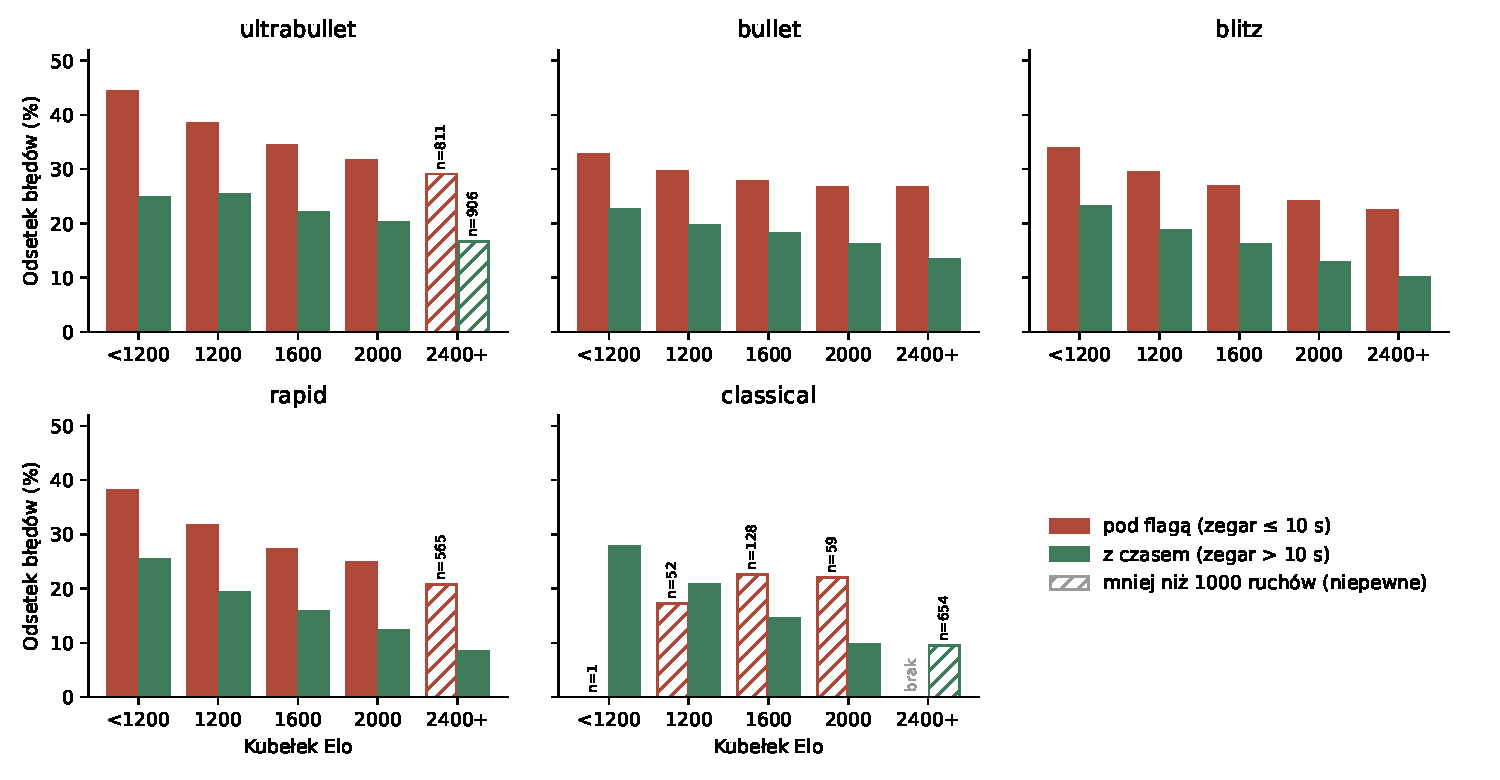
\includegraphics[height=0.78\textheight]{blunder.pdf}\\
\small Pod flagą błędów jest więcej we wszystkich dużych grupach. Kreskowane: $<$1000 ruchów.
\end{frame}

\begin{frame}{Wynik 2: powroty z gorszej pozycji}
\begin{columns}[c]
\column{0.58\textwidth}
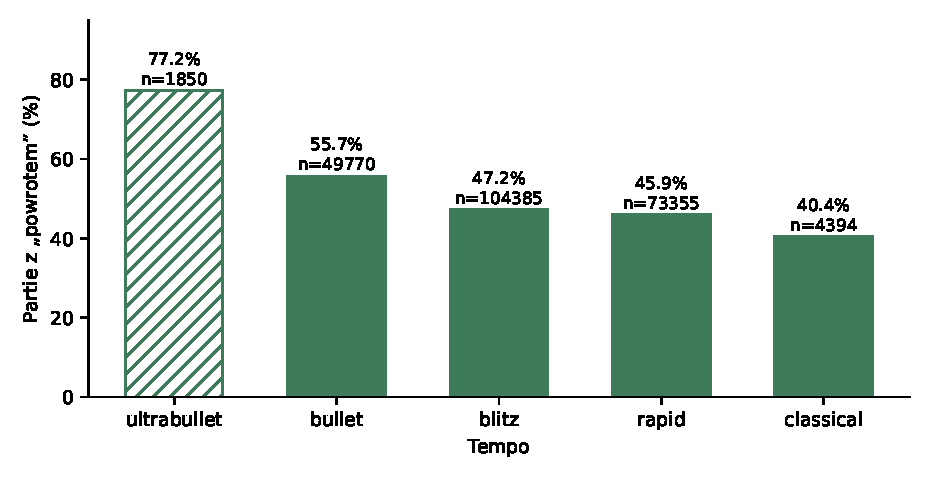
\includegraphics[width=\textwidth]{comeback.pdf}
\column{0.4\textwidth}
\small
\resizebox{\textwidth}{!}{\tabComeback}\\[0.5em]
Im szybsze tempo, tym więcej powrotów, w obu wariantach definicji.\\[0.3em]
To udział partii, nie szansa wygrania z gorszej pozycji.
\end{columns}
\end{frame}

\begin{frame}{Wynik 3: czas namysłu a strata}
\centering
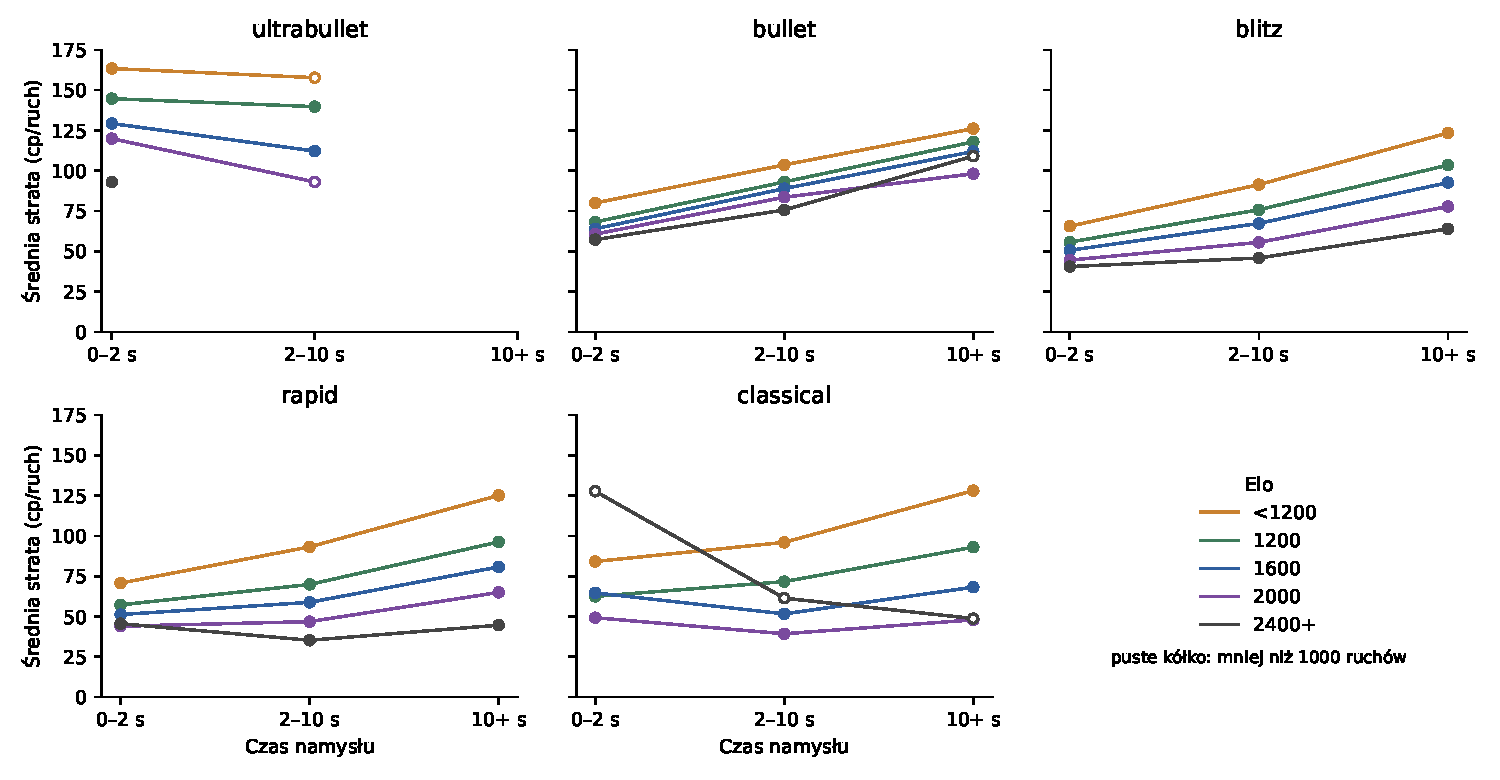
\includegraphics[height=0.78\textheight]{namysl.pdf}\\
\small Blitz i bullet: dłuższy namysł $\to$ większa strata. Korelacja: dłużej myśli się w trudnych pozycjach.
\end{frame}

\begin{frame}{Wnioski i ograniczenia}
\textbf{Wnioski}
\begin{itemize}
\item Presja czasu wyraźnie zwiększa odsetek błędów, najbardziej względnie u najsilniejszych.
\item Powroty są częstsze w szybkich tempach.
\item Długi namysł towarzyszy trudnym pozycjom, a nie lepszym ruchom.
\item Podział wejścia na 8 części: \tOne{} $\to$ \tEight{} (\speedup$\times$ szybciej).
\end{itemize}
\textbf{Ograniczenia}
\begin{itemize}
\item tylko partie z oceną silnika (ok.\ 10\%), początek jednego miesiąca
\item wyniki opisowe i korelacyjne, bez testów istotności
\end{itemize}
\end{frame}

\begin{frame}[fragile]{Demo}
\small
\begin{verbatim}
./run_all.sh --probka              # cały przepływ na 50 MB (~2 min)
docker exec partie-hadoop hdfs dfs -ls -h /user/chess/raw/lichess_2026-09
cat wyniki/full/czasy.tsv          # czasy jobów na 5,5 GB
.venv/bin/python -m src.summary    # liczby dokumentów w obu bazach
.venv/bin/python scripts/check_mongo_tls.py
\end{verbatim}
\normalsize
Panele: NameNode \kod{localhost:9870}, YARN \kod{localhost:8088}.\\
Wykresy: \kod{plots/*.png}. Kod: \kod{github.com/balicz3k/BigData-ChessAnalyzer}.
\end{frame}

\end{document}
